\documentclass[10pt]{article}
\usepackage[a4paper,margin=1.6cm]{geometry}
\usepackage{booktabs}
\usepackage{graphicx}
\usepackage{amsmath}
\usepackage{amssymb}
\pagestyle{empty}
\begin{document}

\section*{E1 physics floor}
\footnotesize
\begin{tabular}{lrrrr}
\toprule
Flight & window & $k_d$ & median residual & drag reduction \\
 & (samples) & (s$^{-1}$) & (deg) & (deg) \\
\midrule
flight-01a-ellipse & 101 & 0.297 & 1.26 & 0.03 \\
flight-04a-ellipse & 101 & 0.298 & 1.19 & -0.00 \\
flight-07a-lemniscate & 101 & 0.297 & 2.94 & 0.01 \\
flight-13a-trackRATM & 101 & 0.297 & 0.96 & 1.14 \\
flight-01p-ellipse & 101 & 0.304 & 0.94 & 5.63 \\
flight-07p-lemniscate & 101 & 0.290 & 0.95 & 5.72 \\
flight-13p-trackRATM & 101 & 0.295 & 3.28 & 3.89 \\
flight-16p-trackRATM & 101 & 0.296 & 3.88 & 3.61 \\
\midrule
Pooled (n = 114,059) & -- & -- & 1.24 & 4.22 \\
\bottomrule
\end{tabular}

\begin{figure}[h]\centering
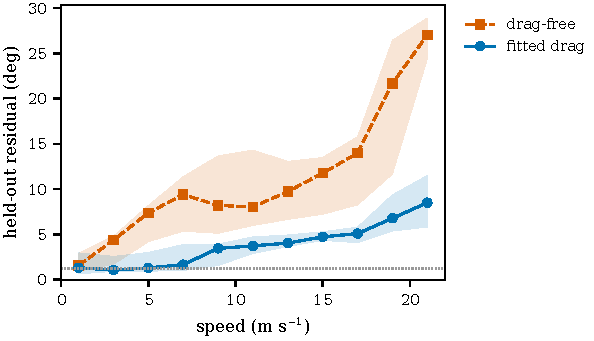
\includegraphics[width=0.5\textwidth]{figures/fig_e1_physics-floor_1.pdf}
\end{figure}

\section*{E2 depicted tilt (TII)}
\footnotesize
\begin{tabular}{llrrrrr}
\toprule
Flight & track & $n$ & median & trimmed RMSE & full RMSE & $>10^\circ$ \\
 & & & (deg) & (deg) & (deg) & (\%) \\
\midrule
flight-01a-ellipse & ellipse & 270 & 4.20 & 4.19 & 13.67 & 10.4 \\
flight-01p-ellipse & ellipse & 1267 & 3.14 & 3.26 & 3.80 & 0.6 \\
flight-04a-ellipse & ellipse & 350 & 3.29 & 3.26 & 10.35 & 5.1 \\
flight-07a-lemniscate & lemniscate & 370 & 2.54 & 6.62 & 28.43 & 17.6 \\
flight-07p-lemniscate & lemniscate & 1284 & 3.59 & 3.71 & 4.20 & 0.5 \\
flight-13a-trackRATM & trackRATM & 557 & 7.44 & 34.63 & 44.36 & 33.4 \\
flight-13p-trackRATM & trackRATM & 536 & 7.85 & 18.44 & 33.69 & 36.4 \\
flight-16p-trackRATM & trackRATM & 373 & 7.34 & 13.56 & 31.18 & 34.9 \\
\midrule
Pooled (all frames) & -- & 5007 & 3.96 & 4.80 & 22.32 & 12.7 \\
\bottomrule
\end{tabular}

\begin{tabular}{lrr}
\toprule
Route & pooled median flight RMSE & frames \\
 & (deg) & \\
\midrule
raw fisheye, \texttt{simple\_divisional} & 13.18 & 192 \\
pinhole, focal prior & 26.90 & 48 \\
pinhole, focal free & 25.41 & 192 \\
\bottomrule
\end{tabular}

\begin{figure}[h]\centering
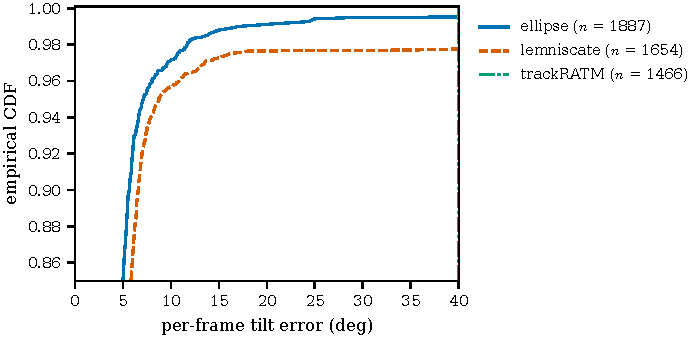
\includegraphics[width=0.5\textwidth]{figures/fig_e2_depicted-tilt-tii_1.pdf}
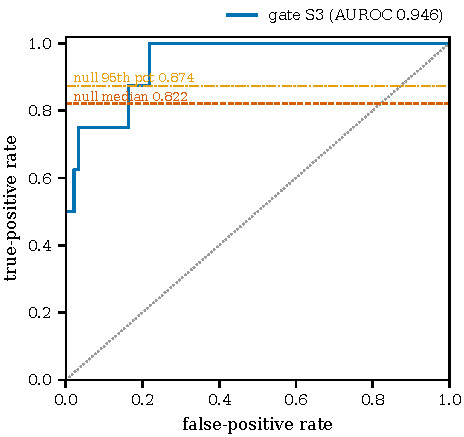
\includegraphics[width=0.5\textwidth]{figures/fig_e2_depicted-tilt-tii_2.pdf}
\end{figure}

\section*{E3 verdict on real flights}
\begin{tabular}{lrrrr}
\toprule
Calibration mode & conformal threshold & fold range & detection floor \\
 & (deg) & (deg) & (deg) \\
\midrule
drag-free, lag-only & 14.73 & [13.50, 16.46] & 15.62 \\
drag-free, full nuisance & 12.95 & [10.61, 13.76] & 13.84 \\
drag 0.295, lag-only & 8.96 & [8.96, 12.07] & 16.62 \\
drag 0.295, full nuisance & 6.46 & [5.84, 10.08] & 16.14 \\
\midrule
\multicolumn{4}{l}{\footnotesize Drag 0.295, full nuisance: cruise null binds at 8.48$^\circ$ (ANWM cruise p99).} \\
\bottomrule
\end{tabular}

\begin{tabular}{lrrr}
\toprule
Flight type & acceptance & abstention & testable real clips \\
 & $k/n$ & (\%) & \\
\midrule
piloted & 51/51 & 21.4 & 51 \\
autonomous & 2/4 & 86.7 & 4 \\
trackRATM & 4/4 & 86.2 & 4 \\
Overall & 57/59 & 41.0 & 59 \\
\bottomrule
\end{tabular}

\begin{figure}[h]\centering
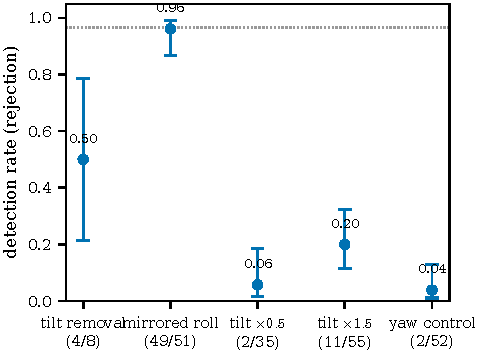
\includegraphics[width=0.5\textwidth]{figures/fig_e3_verdict-real-flights_1.pdf}
\end{figure}

\section*{E4 ANWM data audit}
\footnotesize
\begin{tabular}{llrrrr}
\toprule
Regime & step (s) & per-step, free & per-step, drag & smoothed, free & smoothed, drag \\
\midrule
native paths & 0.250 & 0.00 / 105.50 & 31.02 / 106.07 & 14.62 / 32.93 & 25.64 / 42.00 \\
native paths & 0.667 & 0.00 / 64.73 & 12.71 / 62.37 & 2.26 / 5.61 & 9.20 / 14.36 \\
native paths & 1.000 & 0.00 / 32.63 & 8.55 / 29.64 & 1.01 / 2.48 & 6.11 / 9.15 \\
rescaled racing & 0.250 & 7.59 / 19.72 & 18.05 / 30.34 & 7.55 / 18.71 & 17.93 / 29.48 \\
rescaled racing & 0.667 & 1.05 / 2.87 & 5.57 / 10.92 & 1.05 / 2.71 & 5.58 / 10.83 \\
rescaled racing & 1.000 & 0.47 / 1.28 & 3.62 / 7.22 & 0.47 / 1.20 & 3.63 / 7.16 \\
designed maneuvers & 0.250 & 54.45 / 71.25 & 56.69 / 72.14 & 52.81 / 61.29 & 52.80 / 62.50 \\
designed maneuvers & 0.667 & 11.69 / 23.21 & 16.62 / 26.65 & 10.50 / 14.40 & 15.25 / 18.82 \\
designed maneuvers & 1.000 & 5.26 / 10.79 & 9.83 / 14.57 & 4.71 / 6.51 & 9.30 / 10.72 \\
\bottomrule
\multicolumn{6}{l}{\footnotesize Entries are median / 90th percentile required tilt (deg).} \\
\end{tabular}

\footnotesize
\begin{tabular}{llrrrr}
\toprule
Regime & step (s) & per-step, free & per-step, drag & smoothed, free & smoothed, drag \\
\midrule
native paths & 0.250 & 40.6 & 79.8 & 63.2 & 78.8 \\
native paths & 0.667 & 38.2 & 77.4 & 0.9 & 40.7 \\
native paths & 1.000 & 38.2 & 38.2 & 0.0 & 4.8 \\
rescaled racing & 0.250 & 39.2 & 69.3 & 39.5 & 69.7 \\
rescaled racing & 0.667 & 0.1 & 16.3 & 0.0 & 16.3 \\
rescaled racing & 1.000 & 0.0 & 0.0 & 0.0 & 0.0 \\
designed maneuvers & 0.250 & 87.0 & 100.0 & 85.7 & 99.4 \\
designed maneuvers & 0.667 & 73.9 & 96.4 & 57.8 & 97.4 \\
designed maneuvers & 1.000 & 19.1 & 47.0 & 0.0 & 31.8 \\
\bottomrule
\multicolumn{6}{l}{\footnotesize Fraction of steps with required tilt above $10^\circ$ (\%).} \\
\end{tabular}

\footnotesize
\begin{tabular}{llrrrr}
\toprule
Maneuver & yaw policy & target (deg) & clips & required, free & required, drag \\
\midrule
cruise & course & -- & 7 & 0.00 & 8.55 \\
turn & course & 5 & 3 & 5.00 & 9.83 \\
turn & fixed & 5 & 3 & 5.00 & 9.83 \\
turn & fixed & 10 & 3 & 10.02 & 12.95 \\
turn & fixed & 20 & 3 & 19.94 & 21.19 \\
slalom & course & 5 & 3 & 4.90 & 9.77 \\
slalom & fixed & 5 & 3 & 4.90 & 9.77 \\
slalom & fixed & 10 & 3 & 9.99 & 12.94 \\
accel\_brake & course & 5 & 3 & 4.97 & 12.11 \\
accel\_brake & course & 10 & 3 & 9.90 & 14.88 \\
accel\_brake & course & 20 & 3 & 19.87 & 22.52 \\
climb\_turn & course & 5 & 3 & 5.00 & 9.83 \\
climb\_turn & fixed & 5 & 3 & 5.00 & 9.83 \\
climb\_turn & fixed & 10 & 3 & 10.02 & 12.95 \\
climb\_turn & fixed & 20 & 3 & 19.94 & 21.19 \\
\midrule
\multicolumn{6}{l}{\footnotesize Unreachable designs (at 1 s steps):} \\
turn & course & 10 & -- & 7.44 & 11.20 \\
turn & course & 20 & -- & 7.44 & 11.20 \\
slalom & course & 10 & -- & 7.08 & 10.96 \\
slalom & course & 20 & -- & 7.08 & 10.96 \\
slalom & fixed & 20 & -- & 11.03 & 13.65 \\
climb\_turn & course & 10 & -- & 7.44 & 11.20 \\
climb\_turn & course & 20 & -- & 7.44 & 11.20 \\
\bottomrule
\end{tabular}

\footnotesize
\begin{tabular}{lrrrr}
\toprule
Frames & $n$ & median (deg) & p90 (deg) & $>5^\circ$ (\%) \\
\midrule
512$\times$512 & 186 & 0.57 & 1.62 & 0.5 \\
224$\times$224 & 186 & 0.57 & 1.52 & 0.0 \\
\midrule
\multicolumn{5}{l}{Seed-to-seed pixel MAE: 0.116 (mean of 5 clips, 15 pairs).} \\
\bottomrule
\end{tabular}


\section*{E5 ANWM verdict}
\footnotesize
\begin{tabular}{llrrrr}
\toprule
Mode & interpolant & residual & threshold & margin & margin, strictest fold \\
 & & (deg) & (deg) & (deg) & (deg) \\
\midrule
drag-free lag-only & spline & 20.81 & 14.73 & 3.53 & 1.80 \\
drag-free lag-only & step & 19.02 & 14.73 & 1.98 & 0.25 \\
drag-free full parity & spline & 14.06 & 12.95 & -0.65 & -1.46 \\
drag-free full parity & step & 12.39 & 12.95 & -1.94 & -2.75 \\
$k_d$ 0.295 lag-only & spline & 21.20 & 8.96 & 10.56 & 7.45 \\
$k_d$ 0.295 lag-only & step & 19.54 & 8.96 & 8.84 & 5.72 \\
$k_d$ 0.295 full parity & spline & 14.74 & 8.48 & 5.24 & 3.64 \\
$k_d$ 0.295 full parity & step & 12.86 & 8.48 & 3.78 & 2.18 \\
\bottomrule
\end{tabular}

\footnotesize
\begin{tabular}{llrrr}
\toprule
Cell & mode & clips & infeasible (spline / step) & testable (spline / step) \\
\midrule
Regime A & drag-free lag-only & 8 & -- / -- & -- / -- \\
Regime A & drag-free full parity & 8 & 8/8 / 2/2 & 0/8 / 0/2 \\
Regime A & kd0.295 lag-only & 9 & 9/9 / 2/2 & 0/9 / 0/2 \\
Regime A & kd0.295 full parity & 9 & 9/9 / 2/2 & 0/9 / 0/2 \\
C, 10$^\circ$ & drag-free lag-only & 6 & -- / -- & -- / -- \\
C, 10$^\circ$ & drag-free full parity & 6 & 0/6 / 0/6 & 6/6 / 6/6 \\
C, 10$^\circ$ & kd0.295 lag-only & 6 & 6/6 / 6/6 & 0/6 / 0/6 \\
C, 10$^\circ$ & kd0.295 full parity & 6 & 0/6 / 0/6 & 6/6 / 6/6 \\
C, 20$^\circ$ & drag-free lag-only & 5 & -- / -- & -- / -- \\
C, 20$^\circ$ & drag-free full parity & 5 & 4/5 / 0/5 & 1/5 / 5/5 \\
C, 20$^\circ$ & kd0.295 lag-only & 5 & 5/5 / 5/5 & 0/5 / 0/5 \\
C, 20$^\circ$ & kd0.295 full parity & 5 & 5/5 / 5/5 & 0/5 / 0/5 \\
\bottomrule
\end{tabular}

\begin{figure}[h]\centering
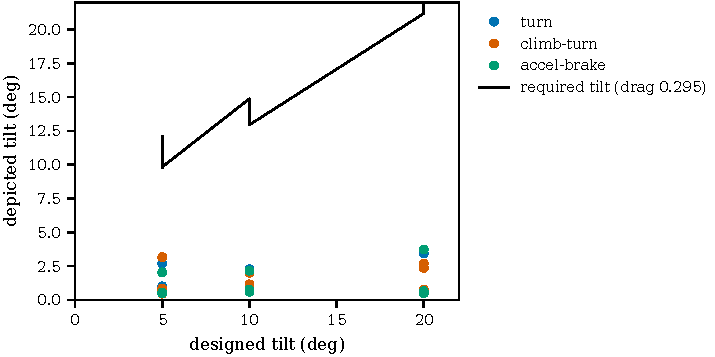
\includegraphics[width=0.5\textwidth]{figures/fig_e5_anwm-verdict_1.pdf}
\end{figure}

\section*{E6 pose injection}
\footnotesize
\begin{tabular}{llrrrr}
\toprule
Maneuver & design (deg) & clips & LPIPS vs level & LPIPS vs prior & prior coverage (mean / min) \\
\midrule
accel\_brake & 5 & 3 & 0.247 & 0.447 & 0.63 / 0.41 \\
accel\_brake & 10 & 3 & 0.176 & 0.490 & 0.58 / 0.28 \\
accel\_brake & 20 & 3 & 0.133 & 0.508 & 0.56 / 0.15 \\
climb\_turn & 5 & 6 & 0.270 & 0.662 & 0.36 / 0.00 \\
climb\_turn & 10 & 3 & 0.394 & 0.555 & 0.53 / 0.36 \\
climb\_turn & 20 & 3 & 0.508 & 0.545 & 0.51 / 0.22 \\
cruise & 0 & 3 & 0.000 & 0.542 & 0.56 / 0.36 \\
slalom & 5 & 6 & 0.182 & 0.528 & 0.55 / 0.35 \\
slalom & 10 & 3 & 0.237 & 0.440 & 0.63 / 0.48 \\
turn & 5 & 6 & 0.223 & 0.629 & 0.39 / 0.00 \\
turn & 10 & 3 & 0.390 & 0.428 & 0.61 / 0.40 \\
turn & 20 & 3 & 0.559 & 0.421 & 0.66 / 0.44 \\
\midrule
Pooled & -- & 45 & 0.266 & 0.534 & -- \\
\bottomrule
\end{tabular}

\begin{figure}[h]\centering
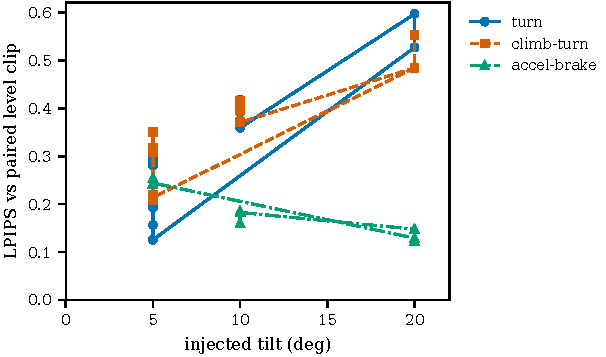
\includegraphics[width=0.5\textwidth]{figures/fig_e6_pose-injection_1.pdf}
\end{figure}
\begin{figure}[h]\centering
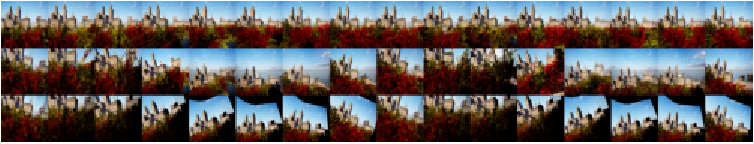
\includegraphics[width=0.8\textwidth]{figures/fig_e6_pose-injection_2.pdf}
\end{figure}

\section*{E7 path from pixels}
\footnotesize
\begin{tabular}{llrrr}
\toprule
Extractor & sequence & direction error & magnitude ratio & pass \\
 & & (deg) & & \\
\midrule
DPVO & indoor\_forward\_3 & 1.78 & 0.98 & yes \\
DPVO & indoor\_forward\_5 & 2.48 & 1.00 & yes \\
DPVO & indoor\_forward\_7 & 20.88 & 0.98 & yes \\
DPVO & indoor\_forward\_9 & 1.45 & 1.00 & yes \\
DPVO & indoor\_forward\_10 & 2.33 & 1.00 & yes \\
DPVO & outdoor\_forward\_1 & 6.75 & 0.94 & yes \\
DPVO & outdoor\_forward\_3 & 5.23 & 0.92 & yes \\
DPVO & outdoor\_forward\_5 & 11.20 & 1.15 & yes \\
DPVO & indoor\_45\_9 & 13.24 & 0.73 & yes \\
DPVO & indoor\_forward\_6 & 3.12 & 0.95 & yes \\
\multicolumn{2}{l}{\textit{DPVO total: 10/10}} & 4.18 & 0.98 & 10/10 \\
\midrule
Pi3 & indoor\_forward\_3 & 22.34 & 1.23 & yes \\
Pi3 & indoor\_forward\_6 & 19.97 & 1.23 & yes \\
Pi3 & indoor\_forward\_5 & 12.52 & 1.12 & yes \\
Pi3 & indoor\_45\_9 & 62.95 & 6.41 & no \\
Pi3 & outdoor\_forward\_5 & 61.96 & 3.76 & no \\
Pi3 & indoor\_forward\_9 & 13.50 & 1.16 & yes \\
Pi3 & indoor\_forward\_10 & 12.10 & 1.10 & yes \\
Pi3 & outdoor\_forward\_1 & 44.30 & 2.36 & no \\
Pi3 & outdoor\_forward\_3 & 31.40 & 1.94 & no \\
Pi3 & indoor\_forward\_7 & 8.40 & 1.10 & yes \\
\multicolumn{2}{l}{\textit{Pi3 total: 6/10}} & 21.16 & 1.23 & 6/10 \\
\midrule
VGGT & indoor\_forward\_3 & 23.32 & 1.28 & yes \\
VGGT & indoor\_forward\_6 & 24.44 & 1.26 & yes \\
VGGT & indoor\_forward\_5 & 28.43 & 1.60 & no \\
VGGT & indoor\_45\_9 & 77.62 & 5.35 & no \\
VGGT & outdoor\_forward\_5 & 76.75 & 3.97 & no \\
VGGT & indoor\_forward\_7 & 22.60 & 1.70 & no \\
VGGT & indoor\_forward\_9 & 28.10 & 1.50 & no \\
VGGT & indoor\_forward\_10 & 30.20 & 1.52 & no \\
VGGT & outdoor\_forward\_1 & 83.80 & 5.98 & no \\
\multicolumn{2}{l}{\textit{VGGT total: 2/9}} & 28.43 & 1.60 & 2/9 \\
\midrule
DA3 & indoor\_forward\_3 & 31.49 & 1.52 & no \\
DA3 & indoor\_forward\_6 & 22.56 & 1.51 & no \\
DA3 & indoor\_forward\_5 & 28.68 & 1.27 & yes \\
DA3 & indoor\_45\_9 & 82.62 & 5.93 & no \\
DA3 & outdoor\_forward\_5 & 58.46 & 4.72 & no \\
DA3 & indoor\_forward\_7 & 25.00 & 1.64 & no \\
DA3 & indoor\_forward\_9 & 28.50 & 1.55 & no \\
DA3 & indoor\_forward\_10 & 18.40 & 1.20 & yes \\
DA3 & outdoor\_forward\_1 & 59.60 & 6.59 & no \\
DA3 & outdoor\_forward\_3 & 55.90 & 4.55 & no \\
\multicolumn{2}{l}{\textit{DA3 total: 2/10}} & 30.08 & 1.59 & 2/10 \\
\bottomrule
\end{tabular}

\begin{tabular}{llrr}
\toprule
Intrinsics fed to DPVO & clips & median direction error (deg) & passing \\
\midrule
fx $\times$ 0.8 & 10 & 12.59 & 9/10 \\
fx $\times$ 0.9 & 10 & 6.60 & 10/10 \\
fx $\times$ 1.0 (calibrated) & 10 & 3.87 & 9/10 \\
fx $\times$ 1.1 & 10 & 8.46 & 9/10 \\
fx $\times$ 1.2 & 10 & 13.45 & 8/10 \\
DA3 estimated K & 10 & 13.54 & 8/10 \\
VGGT estimated K & 10 & 18.86 & 8/10 \\
\bottomrule
\end{tabular}

\begin{tabular}{lr}
\toprule
ANWM outcome (25 clips) & clips \\
\midrule
DPVO crashed & 10 \\
degenerate trajectory (ratio $>10$) & 6 \\
usable & 9 \\
\midrule
Failed verdict pilot (UZH \texttt{indoor\_forward\_5}) & score (deg) \\
\midrule
real & 85.8 \\
tilt-removed & 88.7 \\
\bottomrule
\end{tabular}

\begin{figure}[h]\centering
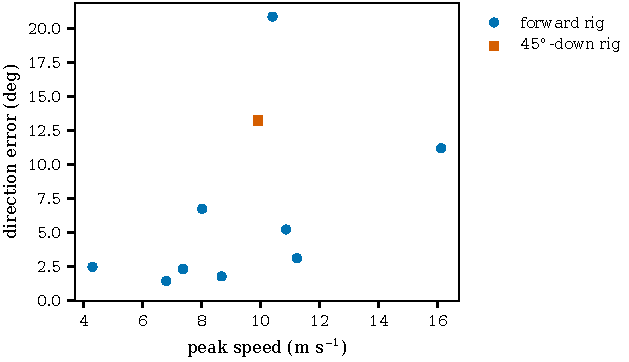
\includegraphics[width=0.5\textwidth]{figures/fig_e7_path-from-pixels_1.pdf}
\end{figure}

\section*{E8 gain and coherence tests}
\begin{tabular}{lrr}
\toprule
Family & gain test & median-residual baseline \\
 & (\%, FRR 5.3\%) & (\%, FRR 3.4\%) \\
\midrule
tilt removal & 100.0 & 67.2 \\
mirrored roll & 100.0 & 94.8 \\
$\times 0.5$ & 100.0 & 17.2 \\
$\times 1.5$ & 96.5 & 24.1 \\
\bottomrule
\end{tabular}

\footnotesize
\begin{tabular}{lrrrr}
\toprule
Flight type & truth to required & estimated to truth & verdict gain & dense required lean \\
 & (slope) & (slope) & (slope) & (slope) \\
\midrule
All clips (57, 6 flights) & 0.991 & 0.828 & 0.745 & 0.764 \\
piloted & 0.997 & 0.831 & 0.753 & 0.770 \\
autonomous & 0.935 & 0.587 & 0.599 & 0.639 \\
track & 0.939 & 0.558 & 0.548 & 0.543 \\
\bottomrule
\end{tabular}

\scriptsize
\begin{tabular}{rrrrrrrr}
\toprule
window (s) & samples & false reject & removal & mirror & $\times 0.5$ & $\times 1.5$ & abstention \\
 & & (\%) & (\%) & (\%) & (\%) & (\%) & (\%) \\
\midrule
0.100 & 27 & 15.8 & 100.0 & 100.0 & 100.0 & 96.5 & 41.0 \\
0.185 & 51 & 8.8 & 100.0 & 100.0 & 100.0 & 96.5 & 41.0 \\
0.370 & 102 & 5.3 & 100.0 & 100.0 & 100.0 & 98.2 & 43.0 \\
0.740 & 203 & 17.5 & 100.0 & 100.0 & 100.0 & 98.2 & 43.0 \\
\bottomrule
\end{tabular}

\begin{tabular}{lrrr}
\toprule
Condition & AUROC (correlation) & detection rate & $n$ \\
\midrule
tilt removal & 0.999 & 100.0 & 57 \\
mirrored roll & 1.000 & 100.0 & 57 \\
$\times 0.5$ & 0.706 & 17.5 & 57 \\
$\times 1.5$ & 0.622 & 24.6 & 57 \\
yaw control & 0.600 & 10.5 & 57 \\
\bottomrule
\end{tabular}

\begin{tabular}{lrrr}
\toprule
Statistic & point & 95\,\% clustered interval & flags (flights) \\
\midrule
Gain tier, pooled & 5.26 \% (3/57) & [2.86, 20.00] & 3 (3 of 6) \\
Gain tier, unweighted mean & 9.67 \% & [0.64, 26.28] & -- \\
\midrule
Coherence, pooled$^\dagger$ & 5.26 \% (3/57) & [0.00, 7.14] & 3 (2 of 6) \\
Coherence, unweighted mean$^\dagger$ & 1.98 \% & [0.00, 4.54] & -- \\
\bottomrule
\end{tabular}

\begin{figure}[h]\centering
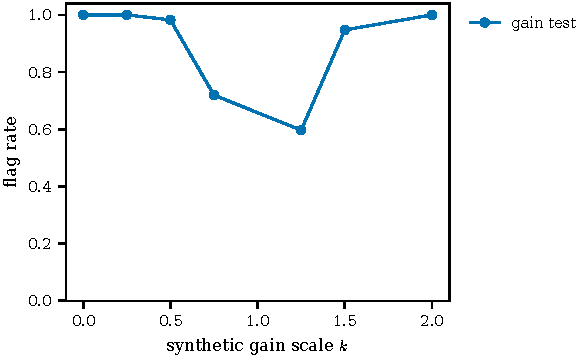
\includegraphics[width=0.5\textwidth]{figures/fig_e8_gain-and-coherence-tests_1.pdf}
\end{figure}

\section*{E9 UZH transfer}
\footnotesize
\begin{tabular}{lrrrrr}
\toprule
Data / variant & $n$ & median & trimmed RMSE & full RMSE & $>10^\circ$ \\
 & & (deg) & (deg) & (deg) & (\%) \\
\midrule
TII reference, raw fisheye & 5007 & 3.96 & 4.80 & 22.32 & 12.7 \\
\midrule
UZH forward, (b) raw fisheye & 3488 & 4.62 & 5.83 & 11.10 & 19.2 \\
UZH forward, (a) pinhole + focal prior & 3488 & 1.53 & 4.29 & 12.66 & 13.1 \\
UZH forward, (c) pinhole, focal free & 3488 & 2.06 & 4.47 & 12.55 & 11.0 \\
\midrule
UZH 45$^\circ$-down, (b) & 5381 & 6.75 & 8.96 & 18.66 & 33.5 \\
\bottomrule
\end{tabular}

\footnotesize
\begin{tabular}{lrrrr}
\toprule
Rig & published elevation & fitted rotation & held-out, published & held-out, fitted \\
 & (deg) & (deg) & (deg) & (deg) \\
\midrule
indoor forward & -0.8 & 3.40 & 3.70 & 2.48 \\
outdoor forward & -0.7 & 35.13 & 9.91 & 10.56 \\
indoor 45 & 45.6 & 14.22 & 10.86 & 5.73 \\
outdoor 45 & 45.9 & -- & -- & -- \\
\bottomrule
\end{tabular}

\begin{tabular}{lr}
\toprule
Sequence & pass rate \\
\midrule
indoor\_forward\_10 & 1.00 (3 pairs) \\
indoor\_forward\_3 & 1.00 (2 pairs) \\
indoor\_forward\_5 & 1.00 (3 pairs) \\
indoor\_forward\_9 & 1.00 (3 pairs) \\
outdoor\_forward\_1 & 0.67 (3 pairs) \\
outdoor\_forward\_3 & 0.67 (3 pairs) \\
outdoor\_forward\_5 & 0.00 (1 pairs) \\
\midrule
All & 18 pairs, overall pass = false \\
\bottomrule
\end{tabular}

\footnotesize
\begin{tabular}{lrrrr}
\toprule
Condition & median residual & R2 band (TII) & coherence tier & $k/n$ (residual) \\
 & (\%) & (\%) & (\%) & \\
\midrule
real false reject & 0.0 & 55.6 & 11.1 & 0/11 \\
null edit & 0.0 & 55.6 & 11.1 & 0/11 \\
yaw control & 0.0 & 28.6 & 14.3 & 0/11 \\
tilt removal & 63.6 & 100.0 & 100.0 & 7/11 \\
mirrored roll & 63.6 & 100.0 & 100.0 & 7/11 \\
$\times 0.5$ & 9.1 & 100.0 & 11.1 & 1/11 \\
$\times 1.5$ & 18.2 & 100.0 & 14.3 & 2/11 \\
\bottomrule
\end{tabular}

\begin{figure}[h]\centering
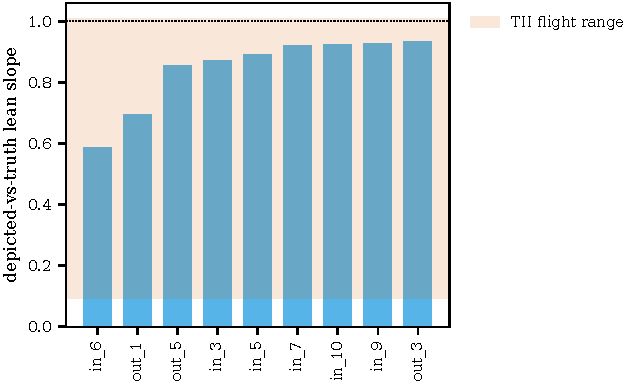
\includegraphics[width=0.5\textwidth]{figures/fig_e9_uzh-transfer_1.pdf}
\end{figure}

\section*{E10 window rule and prototype}
\scriptsize
\begin{tabular}{llrrrrrr}
\toprule
Data & unit & $n$ & truth window & truth samples & clip window & clip samples & floor (truth / clip) \\
 & & & (s) & & (s) & & \\
\midrule
TII & flight-01a-ellipse & 5 & 0.103 & 28.4 & 0.200 & 2.4 & pass / fail \\
TII & flight-01p-ellipse & 26 & 0.178 & 49.0 & 0.286 & 3.4 & pass / fail \\
TII & flight-04a-ellipse & 7 & 0.063 & 17.4 & 0.182 & 2.2 & pass / fail \\
TII & flight-07a-lemniscate & 7 & 0.107 & 29.5 & 0.200 & 2.4 & pass / fail \\
TII & flight-07p-lemniscate & 26 & 0.218 & 59.8 & 0.333 & 4.0 & pass / fail \\
TII & flight-13a-trackRATM & 11 & 0.050 & 13.8 & 0.250 & 3.0 & pass / fail \\
TII & flight-13p-trackRATM & 11 & 0.218 & 59.8 & 0.251 & 3.0 & pass / fail \\
TII & flight-16p-trackRATM & 7 & 0.219 & 60.2 & 0.287 & 3.4 & pass / fail \\
\midrule
UZH forward & indoor\_forward\_10 & 3 & 0.879 & 441.0 & 0.077 & 1.2 & pass / fail \\
UZH forward & indoor\_forward\_3 & 3 & 0.458 & 229.0 & 0.124 & 1.9 & pass / fail \\
UZH forward & indoor\_forward\_5 & 3 & 0.386 & 193.0 & 0.071 & 1.1 & pass / fail \\
UZH forward & indoor\_forward\_6 & 3 & 0.336 & 169.0 & 0.117 & 1.8 & pass / fail \\
UZH forward & indoor\_forward\_7 & 3 & 0.470 & 235.0 & 0.111 & 1.7 & pass / fail \\
UZH forward & indoor\_forward\_9 & 3 & 1.029 & 515.0 & 0.124 & 1.9 & pass / fail \\
UZH forward & outdoor\_forward\_1 & 3 & 1.420 & 711.0 & 0.077 & 1.2 & pass / fail \\
UZH forward & outdoor\_forward\_3 & 3 & 1.339 & 671.0 & 0.111 & 1.7 & pass / fail \\
UZH forward & outdoor\_forward\_5 & 3 & 0.550 & 275.0 & 0.091 & 1.4 & pass / fail \\
\bottomrule
\multicolumn{8}{l}{\footnotesize TII truth rate 274.73 Hz; UZH truth rate 500 Hz; clip rates 12 Hz (TII) and about 15 Hz (UZH).} \\
\end{tabular}

\footnotesize
\begin{tabular}{lrrrrr}
\toprule
Condition & R2 (rule) & coherence (rule) & median residual (rule) & R2 (0.37 s) & coherence (0.37 s) \\
 & (\%) & (\%) & (\%) & (\%) & (\%) \\
\midrule
real false reject & 77.8 (7/9) & 0.0 (0/9) & 0.0 (0/11) & 55.6 (5/9) & 11.1 (1/9) \\
null edit & 77.8 (7/9) & 0.0 (0/9) & 0.0 (0/11) & 55.6 (5/9) & 11.1 (1/9) \\
yaw control & 57.1 (4/7) & 0.0 (0/7) & 0.0 (0/11) & 28.6 (2/7) & 14.3 (1/7) \\
tilt removal & 100.0 (10/10) & 100.0 (10/10) & 63.6 (7/11) & 100.0 (10/10) & 100.0 (10/10) \\
mirrored roll & 100.0 (7/7) & 100.0 (7/7) & 63.6 (7/11) & 100.0 (7/7) & 100.0 (7/7) \\
$\times 0.5$ & 66.7 (6/9) & 11.1 (1/9) & 9.1 (1/11) & 100.0 (9/9) & 11.1 (1/9) \\
$\times 1.5$ & 100.0 (7/7) & 0.0 (0/7) & 18.2 (2/11) & 100.0 (7/7) & 14.3 (1/7) \\
\bottomrule
\end{tabular}

\footnotesize
\begin{tabular}{lrrrl}
\toprule
Case & f95 (Hz) & window (s) & samples & outcome \\
\midrule
smooth curve & 0.0625 & 8.00 & 8.00 & abstain (half duration) \\
slalom & 0.1875 & 2.67 & 2.67 & abstain (floor) \\
straight line & -- & -- & 1.33 & abstain (floor) \\
waypoint step & -- & -- & 1.14 & abstain (floor) \\
\bottomrule
\end{tabular}

\begin{tabular}{llll}
\toprule
Flight type / rig & median residual & gain tier & coherence tier \\
\midrule
TII piloted & validated (57 clips) & calibrated only (57) & validated (57) \\
TII autonomous & calibrated only (4) & not validated (4) & not validated (4) \\
TII trackRATM & not validated (4) & not validated (4) & not validated (4) \\
UZH forward, indoor & validated (9 clips, 4 seq.) & calibrated only (9) & validated (9, 4 seq.) \\
UZH forward, outdoor & not validated & not validated & not validated \\
UZH 45$^\circ$-down & out of scope & out of scope & out of scope \\
\bottomrule
\end{tabular}

\begin{figure}[h]\centering
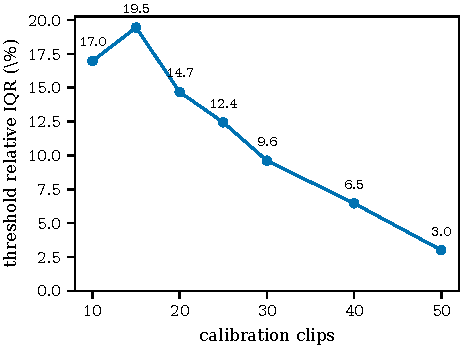
\includegraphics[width=0.5\textwidth]{figures/fig_e10_window-rule-and-prototype_1.pdf}
\end{figure}

\section*{Methodology and reproducibility}
\footnotesize
\begin{tabular}{llllll}
\toprule
Dataset & sensor & rate & truth source & speed / tilt range & used for \\
\midrule
TII racing & fisheye + mocap & mocap 274.73 Hz; camera 12.04 Hz & mocap pose & 6.7-19.1 m/s; tilt median 1-67$^\circ$ & E1-E3, E8, E10 \\
UZH-FPV & forward / 45$^\circ$-down & truth 500 Hz; clips ~15 Hz & sensor ground truth & 4.3-16.1 m/s; tilt median 7-40$^\circ$ & E7, E9, E10 \\
ANWM & generated frames (224/512 px) & 1 s per step, 16 steps & commanded path & required tilt 0-36$^\circ$ & E4-E7 \\
\bottomrule
\multicolumn{6}{l}{\footnotesize Rates, truth sources and ranges from the source audits (phase0 floor, UZH audit, ANWM clip index).} \\
\end{tabular}

\begin{tabular}{llll}
\toprule
Branch & config & commit & sha256 \\
\midrule
track-a-perception & configs/phase1.yaml & e4fd5d9 & c5d3b55e3a2877af \\
track-a2-gate & configs/verdict\_preregistration.yaml & 0834204 & c8ffac93521cbaf2 \\
track-a2-gate & configs/gate\_frozen.yaml & 9e1656d & dc0cc4ff24e0a35d \\
track-c-pathrec & configs/pathrec\_prereg.yaml & 6a16297 & 845f4c698f7a63cc \\
track-d-verdict-stat & configs/gain\_frozen.yaml & 7e8c42e & 28f91f7ffd94c106 \\
track-d-verdict-stat & configs/coherence\_frozen.yaml & 7e8c42e & 40a40beadf372552 \\
track-d-verdict-stat & configs/verdict\_preregistration.yaml & 0834204 & c8ffac93521cbaf2 \\
track-d-verdict-stat & configs/window\_bandwidth\_prereg.yaml & c7af793 & 75b208da5889f133 \\
\bottomrule
\end{tabular}

\footnotesize
\begin{tabular}{llllr}
\toprule
Branch & HEAD & pre-registration / frozen configs & R2 prefix & tests \\
\midrule
track-a-perception & 164c5e0 (2026-11-09) & 1 frozen config(s), see tab\_frozen-configs\_1 & track-a/ & -- \\
track-a2-gate & 428dd3f (2026-11-10) & 2 frozen config(s), see tab\_frozen-configs\_1 & track-a/a2/ & -- \\
track-b-generation & 9ca9e90 (2026-11-10) & -- & track-b/ & -- \\
track-c-pathrec & ed76a08 (2026-11-10) & 1 frozen config(s), see tab\_frozen-configs\_1 & track-c/ & -- \\
track-d-verdict-stat & 2a91765 (2026-11-14) & 4 frozen config(s), see tab\_frozen-configs\_1 & track-d/ & -- \\
track-e-depicted-uzh & dd209bf (2026-11-14) & -- & track-e/ & -- \\
\bottomrule
\end{tabular}


\end{document}
